\documentclass[fontsize=12pt,paper=a4,DIV12,cleardoublepage=empty, 
liststotoc,idxtotoc,bibtotoc]{article}
\usepackage[ngerman]{babel}
\usepackage[utf8]{inputenc}
\usepackage[pdftex]{graphicx}
\usepackage{amsmath}
\usepackage{longtable}
\usepackage{stmaryrd}
\usepackage{colortbl}
\usepackage{eurosym}
\usepackage{amssymb}
\usepackage{amsthm}
\usepackage{nicefrac}
\usepackage{lscape}
\usepackage{pdfpages} 
%Seitenlayout
\renewcommand{\thesection}{\Roman{section}}
\renewcommand{\thesubsection}{\Roman{section}.\arabic{subsection}}
\usepackage[left=25mm, right=25mm, bottom=30mm]{geometry}
\usepackage[doublespacing]{setspace}
\usepackage[colorlinks=true, linkcolor=black, citecolor=black, urlcolor=blue]{hyperref} 
\usepackage[figure]{hypcap}
%Textstruktur
\usepackage{float}
\usepackage{wrapfig}
\usepackage{tabularx}
%Textaussehen
\usepackage{framed}
%Verzeichnisse
\usepackage{csquotes}
\usepackage[backend=biber, bibstyle=authoryear-ibid, uniquelist=false, maxbibnames=9, maxcitenames=3, citestyle=authoryear-icomp, isbn=true, url=true, block=space, pagetracker=page,   giveninits=false, dateabbrev=false, dashed=false ]{biblatex}
\addbibresource{MA_literatur.bib}
\DefineBibliographyStrings{ngerman}{ 
	andothers = {{et\,al\adddot}},             
} 
\usepackage{etoolbox}
\apptocmd{\UrlBreaks}{\do\f\do\m}{}{}
\setcounter{biburllcpenalty}{9000}% Kleinbuchstaben
\setcounter{biburlucpenalty}{9000}% Großbuchsta
\expandafter\def\expandafter\quote\expandafter{\quote\small\singlespacing}

\setcounter{section}{0}
\setcounter{subsection}{0}

\newcommand*{\meincite}[1]{\citeauthor{#1} (\citeyear{#1})}

\newcommand{\KK}{\mathbb{•}{K}}
\newcommand{\CC}{\mathbb{C}}
\newcommand{\RR}{\mathbb{R}}
\newcommand{\QQ}{\mathbb{Q}}
\newcommand{\ZZ}{\mathbb{Z}}
\newcommand{\NN}{\mathbb{N}}
\newcommand{\PPO}{\mathcal{P}(\Omega)}

\theoremstyle{plain}
\newtheorem{satz}{Satz}[subsection]
\newtheorem{lem}[satz]{Lemma}
\newtheorem{theo}[satz]{Theorem}
\newtheorem{kor}[satz]{Korollar}
\newtheorem{defi}{Definition}
\theoremstyle{definition}
\newtheorem{bei}[satz]{Beispiel}
\newtheorem{bem}[satz]{Bemerkung}

\graphicspath{ {./images/} }

\begin{document}
	\definecolor{gold}{rgb}{0.9,0.9,0}
	\begin{titlepage}
		\vspace*{-3cm}
		\noindent
		\hspace*{1cm}
			\begin{center}
				\centering
				{\LARGE Gesamtschule Scharnhorst}
			\end{center}
		\begin{center}
		\Large{Fundamentalsatz der Analysis}\\[0.5cm]
		\normalsize{geschrieben von}\\[0.25cm]	
		\large{Benno Schörmann}\\[0.5cm]
		\end{center}
	\begin{flushleft}
	\hyperref[subsec:thema1]{\textbf{\large Thema der Facharbeit:}}  \\
	\end{flushleft}
	Eine vollständige Definition und ein vollständiger Beweis des Fundamentalsatzes der Analysis
	\vfill
	\vfill
	\begin{tabular}{r}
	\Large{18.03.2022}\normalsize
	\end{tabular}
	\hfill
	\quad \\[1.5cm]
	\noindent 
	\renewcommand{\arraystretch}{1.4}
	\end{titlepage}
	\newpage
	\thispagestyle{empty}
	\tableofcontents
	\newpage
	%\listoffigures
	%\thispagestyle{empty}
	%\newpage	
	%\section{Einleitung}
	%(Die Einteilung steht übrigens noch absolut nicht fest, habe sie gestern abend im Halbschlaf angefertigt) \\\\
	%In dieser Facharbeit werde ich über Den Fundamentalsatz der Analysis und die dazugehörigen Nebenpunkte schreiben.
	
	
	
	\section{Geschichtliche Zusammenfassung}
	Genutzte Quellen: [\cite[vgl.]{DMB}]\\
	Die Geschichte des Hauptsatzes der Differential- und Integralrechnung beginnt im 17. Jahrhundert mit Gottfried Leibniz und Isaac Newton. Leibniz sah das Integral als eine unendlich große Menge an Flächen die unendlich klein sind. Damit zeigte er den wichtigen Zusammenhang zwischen Integration und Fläche. Isaac Newton nutzte die Geometrie, um den Unterschied zwischen Distanz, Geschwindigkeit und Beschleunigung zu beschreiben. Das ist der Schlüssel, um das Verhältnis zwischen Integral und Ableitung zu verstehen. Krümmung ist die Ableitung von Steigung und Steigung ist die Ableitung von Strecke/Distanz. Distanz ist hingegen das Integral von Steigung und Steigung ist das Integral von Krümmung. 1823 hat Cauchy das Integral per Limes definiert. Im 19. Jahrhundert beschrieb Siméon Denis Poisson das bestimmte Integral als die Differenz der Stammfunktion [F(b)-F(a)]. Um 1950 wurden die Theorien zu einem Hauptsatz der Differential- und Integralrechnung zusammengefasst.
\newpage
	
	

	%\section{Alle wichtigen Begriffe erklärt}
	%Anschauliche Beispiele? (Scipy Einbindung?)
	
	
	%\subsection{Was ist Differentialrechnung?}
	%-eines der am einfachsten zu begreifenden Themen der Analysis ermöglicht dieser Teil der Analysis das finden von Extrema und das generelle Beschreiben von Funktionsverläufen.
	
	
	%\subsubsection{Wie wird eine Funktion abgeleitet?}
		%Text
	
	
	%\subsection{Was ist Integralrechnung?}
		%Text


	%\subsubsection{Wie wird eine Funktion integriert?}
		%Text \cite{KW}
		
	
	%\subsection{Was ist eine stetige Funktion?}
		%Text	
	
	\section{Riemann-Integral}	
	Flächen von Funktionen können mit dem Riemann-Integral approximiert werden. Dies geschieht, indem das Intervall $[a, b]$ in viele kleinere Partitionen $[x_0, x_1, x_2 \cdots x_{k-2}, x_{k-1}, x_k]$ unterteilt wird, wobei $x_0 = a$, $x_k = b$ und $[x_0 < x_1 < x_2 < \cdots < x_{k-2} < x_{k-1} < x_k]$. Bei gegebener Funktion $f \in \RR$ wird nun die Höhe von $f(x_k)$ oder $f(x_{k-1})$ mit der Breite $(x_k-x_{k-1})$ oder einfachheitshalber $\Delta x$ multipliziert. Nun wird entweder nur der höchste Wert zwischen $f(x_k)$ und $f(x_{k-1})$ ausgewählt, was die Obersumme wäre oder der tiefste Wert zwischen $f(x_k)$ und $f(x_{k-1})$ ausgewählt, was die Untersumme wäre.\\
	 In Form einer Gleichung bedeutet das
	\begin{equation*}
		O(Z)= \sum_{k=1}^{n} [(\Delta x)* \sup_{x_{k-1} \leq x \leq x_k} f(x)]
	\end{equation*}
	\begin{equation*}
		U(Z)= \sum_{k=1}^{n} [(\Delta x)* \inf_{x_{k-1} \leq x \leq x_k} f(x)]
	\end{equation*}
	Da, wie im unteren Bild zu sehen ist, der Graph ausschließlich zwischen der Ober- und Untersumme verläuft können mehrere Schlüsse gezogen werden. Erstens ist das Integral irgendein Wert zwischen Ober- und Untergrenze und somit eingegrenzt mit einer bekannten Ungenauigkeit. Zweitens, wenn Obergrenze = Untergrenze ist, ist das Integral exakt bestimmt, da der Bereich zwischen Ober- und Untergrenze gleich 0 ist, was bedeutet, dass der Graph exakt zwischen den Grenzen verläuft. \\Eine andere Schreibart für die Untergrenze ist
	\begin{equation*}
	\underline{\int _{a}^{b}}f(x)dx
	\end{equation*}
	Eine andere Schreibart für die Obergrenze ist
	\begin{equation*}
	\overline{\int _{a}^{b}}f(x)dx
	\end{equation*}
	Somit folgt aus der oberen Feststellung, dass wenn
	\begin{equation*}
		\underline{\int _{a}^{b}}f(x)dx = \overline{\int _{a}^{b}}f(x)dx
	\end{equation*}
	dann
	\begin{equation*}
		\underline{\int _{a}^{b}}f(x)dx = \overline{\int _{a}^{b}}f(x)dx = \int_{a}^{b}f(x)dx
	\end{equation*}
	\\\\ Hier ein bildliches Beispiel der Ober- und Untersummen:\\
	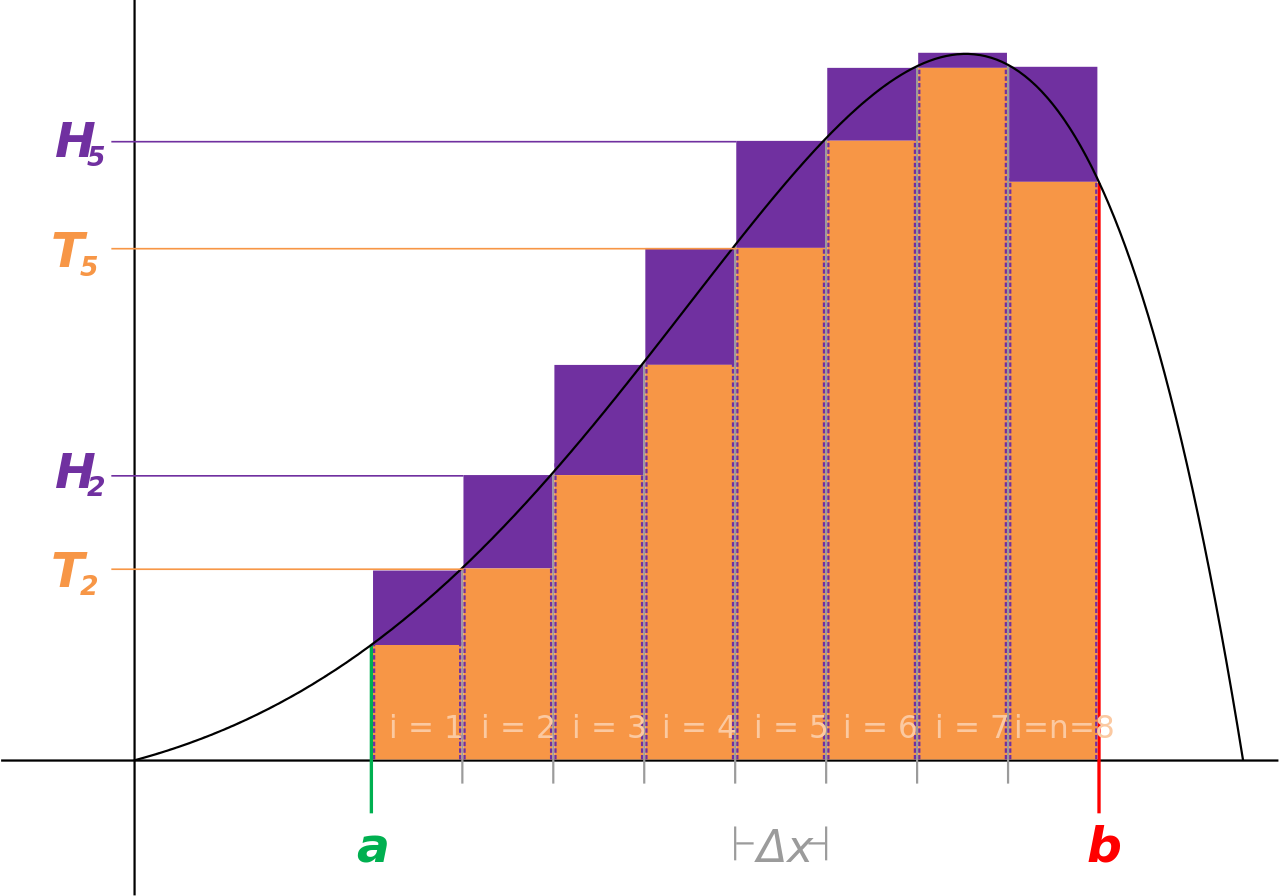
\includegraphics[scale=0.3]{Riemann.png}
	
	
	\section{Mittelwertsatz der Integralrechnung}
	Genutzte Quellen: [\cite[vgl.]{MWS}]
	\begin{satz}" "\\
		Gegeben ist die in $\RR$ definierte Funktion auf dem Intervall $[a, b]$ liegende Funktion $f$ und $g$. $g$ ist außerdem integrierbar und ohne Vorzeichenwechsel, also $g \geq 0$ \textbf{oder} $g \leq 0$. Dann existiert mindestens ein $\xi$, sodass
		\begin{equation*}
			\int_{a}^{b}f(t)g(t)dt=f(\xi)\int_{a}^{b}g(t)dt			
		\end{equation*}
		Die obige Aussage wird auch als erweiterter Mittelwertsatz bezeichnet. Wenn allerdings $g=1$ ist, kommt es zu einem Spezialfall\\
		%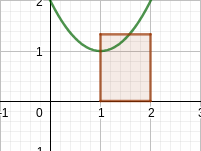
\includegraphics[scale=0.3]{Mittelwertsatz xTo2.png}
		\begin{equation*}
			\int_{a}^{b}f(t)dt=f(\xi)(b-a)
		\end{equation*}
		Wenn die rechte Seite der Gleichung betrachtet wird, fällt auf, dass dort der eines Rechtecks gebildet wird. Dieses Rechteck hat die gleiche Fläche wie das Integral zwischen $a$ und $b$.		
		
	\end{satz}
	
	\begin{proof}" "\\
		Gegeben ist die in $\RR$ definierte Funktion $g$, wobei $g(x)\geq0$ und auf dem Intervall $[a, b]$ liegt.\\
		$f$ nimmt zwischen $a$ und $b$ ein Minimum $k$ und ein Maximum $K$ an. Somit ist $k \leq f(x) \leq K$ und bei $g\geq0$ ist $kg(x)\leq f(x)g(x)\leq Kg(x)$. Daraus erschließt sich
		\begin{equation*}
			k \int_{a}^{b}g(x)dx \leq \int_{a}^{b}f(x)g(x)dx\leq K\int_{a}^{b}g(x)dx
		\end{equation*}
		Es gilt nun zwischen zwei Fällen zu unterscheiden.\\
		\textbf{Fall 1:} $\int_{a}^{b}g(x)dx \neq 0$, dann
		\begin{equation*}
			f(\xi)=\frac{1}{\int_{a}^{b}g(x)dx}\int_{a}^{b}f(x)g(x)dx
		\end{equation*}
		Die rechte Seite dieser Gleichung ist eine Zahl, und zu zeigen ist, dass $f$ für ein $\xi \in [a, b]$ diese Zahl als Wert annimmt.\\	
		Wegen $g(x) \geq 0$ ist $\int_{a}^{b}g(x)dx > 0$ und hat nach der Division durch $\int_{a}^{b}g(x)dx$ die Form
		\begin{equation*}
			k \leq \frac{1}{\int_{a}^{b}g(x)dx}\int_{a}^{b}f(x)g(x)dx \leq K
		\end{equation*}
		hieraus folgt mit dem Zwischenwertsatz für stetige Funktionen, q. e. d.\\
		\textbf{Fall 2:} $\int_{a}^{b}g(x)dx = 0$, dann 
		\begin{equation*}
			 \int_{a}^{b}f(x)g(x)dx = 0
		\end{equation*}
		und die Behauptung gewinnt die für jedes $\xi \in [a, b]$ gültige Form.
	\end{proof}
	\newpage
	
	
	\section{Hauptsatz der Differential- und Integralrechnung}
	
	Der Hauptsatz der Differential- und Integralrechnung ist in zwei Hauptsätze und einen Nebensatz aufgeteilt. Der erste Satz stellt den Zusammenhang zwischen Integral und Differential dar.

	\subsection{Erster Teil}
	\begin{satz}" "\\
		Gegeben ist die in $\RR$ definierte Funktion $f$ in einem geschlossenen Intervall $[a, b]$. Sei $F$ definiert für alle $x$ im Intervall $[a, b]$ durch \\
			\begin{equation*}
				F(x)=\int_{a}^{x}f(t) dt
			\end{equation*}
		Dann ist $F$ gleichmäßig stetig auf dem Intervall $[a, b]$ und differenzierbar auf dem offenen Intervall $(a, b)$, und 
			\begin{equation*}
				F'(x)=f(x)
			\end{equation*}
		Für alle $x$ in $(a, b)$, sodass $F$ eine Stammfunktion von $f$ ist.\\
	\end{satz}
	
	\begin{proof}" "\\
		Für ein gegebenes $f(t)$ sei die Funktion $F(x)$ definiert als
		\begin{equation*}
			F(x)=\int_{a}^{x}f(t)dt
		\end{equation*}
		Für jegliche 2 Zahlen $x_1$ und $\Delta x$ im Intervall $[a, b]$ ergibt sich
		\begin{equation*}
			F(x_1)=\int_{a}^{x_1}f(f)dt
		\end{equation*}
		und
		\begin{equation*}
			F(x_1+\Delta x)=\int_{a}^{x_1+\Delta x}f(t)dt
		\end{equation*}
		Wenn diese beiden Gleichungen nun subtrahiert werden, dann ergibt sich
		\begin{equation}
			F(x_1+\Delta x)-F(x_1)=\int_{a}^{x_1+\Delta x}f(t)dt-\int_{a}^{x_1}f(t)dt
		\end{equation}
		Die Summe beider Flächen ist
		\begin{equation*}
			\int_{a}^{x_1}f(t)dt + \int_{x_1}^{x_1+\Delta x}f(t)dt = \int_{a}^{x_1+\Delta x}f(t)dt
		\end{equation*}
		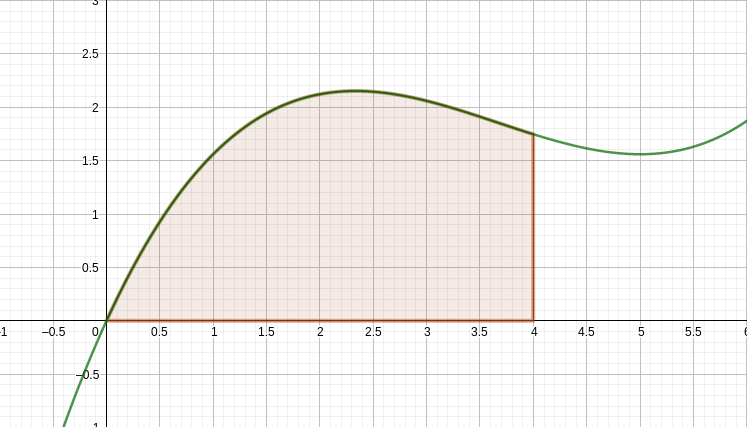
\includegraphics[scale=0.2]{Integral 0-4.png} $+$
		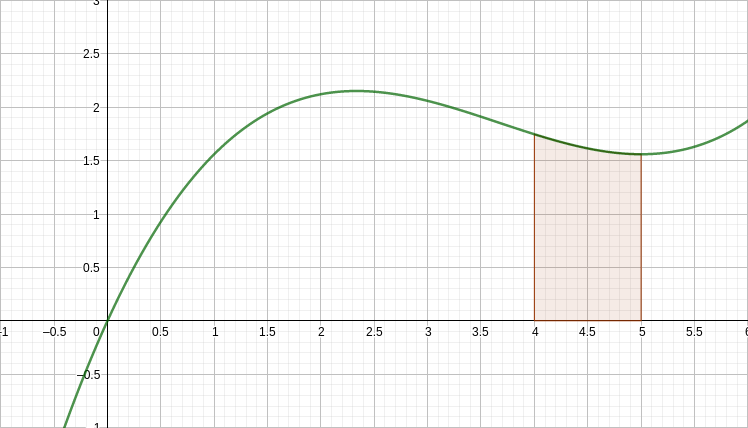
\includegraphics[scale=0.2]{Integral 4-5.png} $=$
		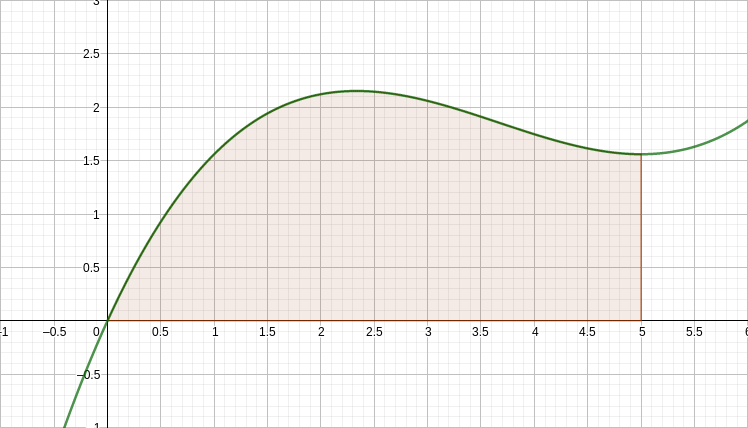
\includegraphics[scale=0.2]{Integral 0-5.png} \\
		Wenn, wie in dem oben gezeigten Fall, die Flächen zweier Integrale von z.B. 0 bis 4 und 4 bis 5 addiert werden, dann ergibt das die Fläche des Integrals von 0 bis 5. Generell ausgedrückt ist das also
		\begin{equation*}
			\int_{a}^{b}f(t)dt + \int_{b}^{c}f(t)dt = \int_{a}^{c}f(t)dt
		\end{equation*}
		, wobei $a\leq b\leq c$.\\
		Die Umformung dieser Gleichungen gibt
		\begin{equation*}
			\int_{a}^{x_1+\Delta x}f(t)dt-\int_{a}^{x_1}f(t)dt=\int_{x_1}^{x_1+\Delta x}f(t)dt
		\end{equation*}
		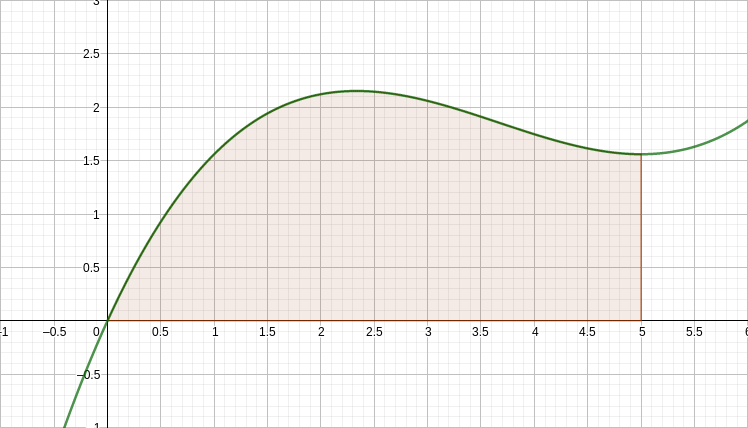
\includegraphics[scale=0.2]{Integral 0-5.png} $-$
		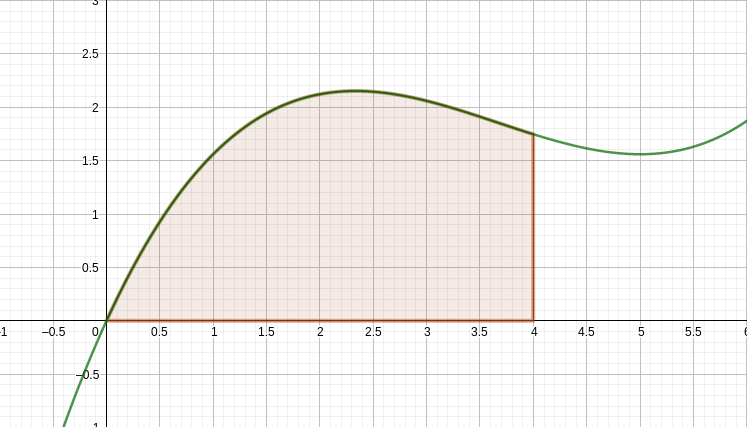
\includegraphics[scale=0.2]{Integral 0-4.png} $=$
		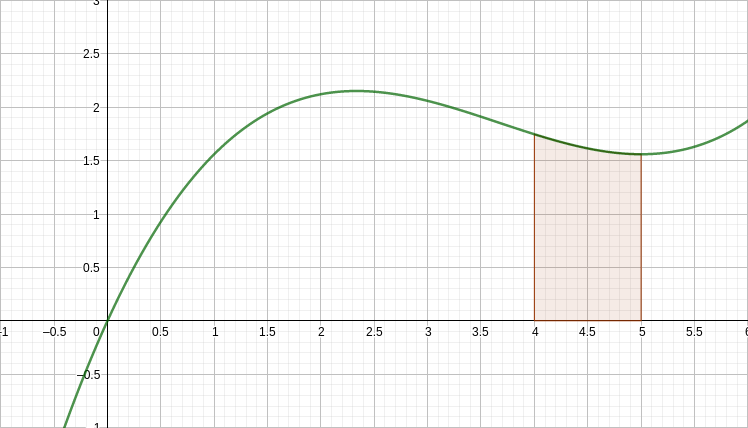
\includegraphics[scale=0.2]{Integral 4-5.png} \\
Wenn, wie in dem oben gezeigten Fall, die Flächen zweier Integrale von z.B. 0 bis 5 und 0 bis 4 voneinander subtrahiert werden, dann ergibt das die Fläche des Integrals von 4 bis 5. Generell ausgedrückt ist das also
		\begin{equation*}
			\int_{a}^{c}f(t)dt - \int_{a}^{b}f(t)dt = \int_{b}^{c}f(t)dt
		\end{equation*}
		, wobei $a\leq b\leq c$.\\
		Nun wird die Gleichung (1) eingesetzt.
		\begin{equation}
			F(x_1+\Delta x)-F(x_1)=\int_{x_1}^{x_1+\Delta x}f(t)dt
		\end{equation}
		Laut dem Mittelwertsatz der Integralrechnung gibt es eine Zahl c in $[x_1, x_1+\Delta x]$, sodass
		\begin{equation}
			\int_{x_1}^{x_1+\Delta x}f(t)dt=f(c)*\Delta x
		\end{equation}
		Nun wird die Gleichung (2) und (3) zusammengefügt und durch $\Delta x$ dividiert
		\begin{equation*}
			F(x_1+\Delta x)-F(x_1)=f(c)*\Delta x \;\;\;\;|\div \Delta x
		\end{equation*}
		\begin{equation*}
			\frac{F(x_1+\Delta x)-F(x_1)}{\Delta x}=f(c)
		\end{equation*}
		Auffallend ist, dass die linke Seite zu einem Differenzeinquotienten umgeformt wurde. Wird nun $\lim \limits_{\Delta x \to 0}$ angewandt, dann
		\begin{equation*}
			\lim \limits_{\Delta x \to 0} \frac{F(x_1+\Delta x)-F(x_1)}{\Delta x}=\lim \limits_{\Delta x \to 0}f(c)
		\end{equation*}
		Und somit
		\begin{equation}
			F'(x_1)=\lim \limits_{\Delta x \to 0}f(c)
		\end{equation}
		Nun fehlt nur noch $f(c)$.\\ Da $x_1 \leq c \leq x_1+\Delta x$ ist und $\Delta x$ gegen $0$ läuft wird sich $c\to$ $x_1$ nähern bis bei $\Delta x=0$ auch $c = x_1$ ist, beziehungsweise $x_1 \leq c \leq x_1 + 0$ oder $x_1 = c = x_1$ ist.\\Zusammenfassend ist also
		\begin{equation}
			\lim \limits_{\Delta x \to 0} f(c) = f(x_1)
		\end{equation}
		Und somit, wenn (4) und (5) zusammenfügt werden
		\begin{equation*}
			F'(x_1)=f(x_1)
		\end{equation*}
		Eine andere Schreibweise wäre
		\begin{equation*}
			\frac{d}{dx}\int_{a}^{x}f(t)dt=f(x)
		\end{equation*}
		Damit ist der erste Satz der Differential- und Integralrechnung bewiesen.
	\end{proof}
	\newpage
	
	
	\subsection{Korollar}
	\begin{satz}" "\\
		Gegeben ist die in $\RR$ definierte, auf dem Intervall $[a, b]$ stetige Funktion $f$  und $F$ eine Stammfunktion von $f$ im Intervall $[a, b]$, dann gilt
		\begin{equation*}
			\int_{a}^{b}f(t)dt=F(b)-F(a)
		\end{equation*}
		Das Korollar erfordert Stetigkeit auf dem ganzen Intervall.
	\end{satz}

	\begin{proof}" "\\
		Sei $F$ ein Stammfunktion von $f$ mit Stetigkeit auf dem Intervall $[a, b]$, dann sei
		\begin{equation*}
			G(x)=\int_{a}^{x}f(t)dt
		\end{equation*}
		Durch den ersten Beweis ist bewiesen, dass $G(x)$ eine Stammfunktion von f ist. Da $F'(x)-G'(x)=0$ ist der Mittelwertsatz der Integralrechnung impliziert, dass $F(x)-G(x)$ eine konstante Funktion ist, das heißt es gibt eine Zahl $c$, so dass $G(x)=F(x)+c$ für alle $x$ in $[a, b]$. Es gilt also
		\begin{equation*}
			F(a)+c=G(a)=\int_{a}^{a}f(t)dt=0
		\end{equation*}
		Das bedeutet, dass $c=-F(a)$. In anderen Worten, $G(x)=F(x)-F(a)$, und somit
		\begin{equation*}
			\int_{a}^{b}f(t)dt=G(b)=F(b)-F(a)
		\end{equation*}
		Somit ist das Korollar des Hauptsatzes der Differential- und Integralrechnung bewiesen.
	\end{proof}	
	\newpage
	
	
	\subsection{Zweiter Teil}
	Genutzte Quellen: [\cite[vgl.]{SPM}]
	\begin{satz}" "\\
	Dieser Teil wird manchmal Zweiter Teil des Hauptsatzes der Differential- und Integralrechnung oder das Newton-Leibniz-Axiom genannt.\\
	Gegeben ist die in $\RR$ definierte Funktion $f$ auf dem geschlossenen Intervall $[a, b]$, und $F$, eine Stammfunktion von $f$ auf dem Intervall $(a, b)$
	\begin{equation*}
		F'(x)=f(x)
	\end{equation*}
	Wenn $f$ auf dem Intervall $[a, b]$ Riemann-integrierbar ist, dann 
	\begin{equation*}
		\int_{a}^{b}f(x)dx=F(b)-F(a)
	\end{equation*}
	Der zweite Teil ist aussagekräftiger als das Korollar, da er nicht voraussetzt, dass $f$ eine stetige Funktion ist.\\
	Wenn eine Stammfunktion $F$ von $f$ existiert, dann gibt es unendlich viele unterschiedliche Stammfunktionen die erlangt werden, indem eine Konstante, oftmals $c$ genannt, an $F$ addiert wird. Außerdem existiert laut dem ersten Teil eine Stammfunktion $F$, sobald $f$ kontinuierlich ist, was durch das nicht Vorhandensein einer Stammfunktion von Funktionen, wie $e^{-x^2}$ widerlegt ist.
	
	\end{satz}	
	
	\begin{proof} " "\\
	Dies ist ein Grenzbeweis durch die Riemann-Summe. Sei $f$ Riemann-integrierbar auf dem Intervall $[a, b]$ und lasse $f$ eine Stammfunktion $F$ auf dem Intervall $[a,b]$ zu. $F(b)-F(a)$. Seien $x_0 \cdots x_n$, sodass
	\begin{equation*}
		a = x_0 < x_1 < x_2 < \cdots < x_{n-2} < x_{n-1} < x_n = b
	\end{equation*}
	Daraus lässt sich erschließen, dass
	\begin{equation*}
		F(b)-F(a)=F(x_n)-F(x_0)
	\end{equation*}
	\newpage
	Nun wird jedes $F(x_k)$ zusammen mit seinem negativen gegenpart addiert, sodass die daraus ergebende menge folgendes ergibt
	\begin{multline*}
	\begin{aligned}
		F(b)-F(a)=& F(x_n)+[-F(x_{n-1})+F(x_{n-1})]+[-F(x_{n-2})+F(x_{n-2})]+\cdots +\\ &[-F(x_2)+F(x_2)]+[-F(x_1)+F(x_1)]-F(x_0)\\
		=& [F(x_n)-F(x_{n-1})]+[F(x_{n-1})-F(x_{n-2})]+\cdots+[F(x_2)-F(x_1)]+[F(x_1)-F(x_0)]
	\end{aligned}
	\end{multline*}
	Die obere Menge kann folgendermaßen zusammengefasst werden
	\begin{equation}
		F(b)-F(a)=\sum_{k=1}^{n} [F(x_k)-F(x_{k-1})]
	\end{equation}
	Als nächstes wird der Mittelwertsatz der Integralrechnung benötigt. Kurz zusammengefasst:\\
	Sei $F$ stetig auf dem geschlossenen Intervall $[a, b]$ und differenzierbar auf dem offenen Intervall $(a, b)$, dann existiert ein $c$ im Intervall $(a, b)$, sodass 
	\begin{equation*}
		F'(c)=\frac{F(b)-F(a)}{b-a}
	\end{equation*}
	Daraus folgt
	\begin{equation*}
		F'(c)(b-a)=F(b)-F(a)
	\end{equation*}
	$F$ ist differenzierbar auf dem Intervall $[a, b]$ und somit auch differenzierbar auf dem Intervall $[x_{k-1}, x_k]$. Laut dem Mittelwertsatz der Integralrechnung ergibt sich somit
	\begin{equation}
		F(x_k)-F(x_{k-1})=F'(c_k)(x_k-x_{k-1})
	\end{equation}
	Nun wird das Ergebnis von (7) in die Gleichung von (6) eingesetzt
	\begin{equation*}
		F(b)-F(a)=\sum_{k=1}^{n} [F'(c_k)(x_k-x_{k-1})]
	\end{equation*}
	Vorausgesetzt wird, dass $F'(c_k)=f(c_k)$ ist. Außerdem kann einfachheitshalber $(x_k-x_{k-1})$ als $\Delta x$ des Teils $k$ geschrieben werden, also $\Delta x_k$
	\begin{equation}
		F(b)-F(a)=\sum_{k=1}^{n} [f(c_k)(\Delta x_k)]
	\end{equation}
	\newpage
Mit dem oberen Ausdruck in der Summe wird die Fläche eines Rechtecks mit der Breite $\Delta x$ und Höhe $f(c_k)$ beschrieben. Diese Fläche ist eine Annäherung der Fläche unter dem Graphen $f$ jeder Partition. Jede einzelne Partition wird nun addiert, um sich der Fläche unter der Funktion $f$ im Intervall $[a, b]$ anzunähern. Je kleiner $\Delta x$ wird, desto genauer spiegeln die Rechtecke die Fläche unter der Funktion wieder, da es weniger Unter- oder Überschuss gibt. Wenn in der Theorie $\Delta x = 0$ erreicht ist,dann  würde die exakte Fläche herauskommen. Da in dem Falle die Höhe von $f$ aber immer mit $0$ addiert werden würde, also $0$ herauskommen würde, und $b$ niemals erreicht werden würde ist dies in der Praxis natürlich nicht umzusetzen.\\
	Deswegen wird Limes $\Delta x_k \to 0$ angewendet. Dies bewirkt, dass die Partitionen gen 0 gehen und die Genauigkeit des Intervalls immer besser wird, da es immer weniger Ungenauigkeiten gibt.
	\begin{equation*}
		\lim \limits_{\Delta x_k \to 0} F(b)-F(a)=\lim \limits_{\Delta x_k \to 0} \sum_{k=1}^{n} [f(c_k)(\Delta x_k)]
	\end{equation*}
	Da $F(b)-F(a)$ kein $\Delta x_k$ beinhaltet bleibt diese Seite der Gleichung unverändert bestehen und somit bleibt
	\begin{equation*}
		F(b)-F(a)=\lim \limits_{\Delta x_k \to 0} \sum_{k=1}^{n} [f(c_k)(\Delta x_k)]
	\end{equation*}
	Die rechte Seite der Gleichung definiert das Integral von $f$ von $a$ bis $b$. Somit ergibt sich
	\begin{equation*}
		F(b)-F(a)=\int_{a}^{b}f(x)dx
	\end{equation*}
	Somit ist der Zweite Teil des Hauptsatzes der Differential- und Integralrechnung bewiesen.
	\end{proof}
	
	
	
	\section{Fazit}
	Die oben aufgestellten Beweise zeigen, dass Integral und Ableitung jeweils wie Plus und Minus oder Mal und Geteilt gegensätzliche Vorgehen sind, um Graphen zu analysieren. Zusätzlich wurde bewiesen, wie die Stammfunktion genutzt werden kann, um das Integral zwischen zwei Stellen mit einer Rechnung exakt zu berechnen. Die Beweise bilden Grundlegende Feststellungen, auf denen viele Themen aufbauen, die teilweise sogar außerhalb der Mathematik angewandt werden. Bei Künstlicher Intelligenz werden zum Beispiel Ableitungen benutzt, um Neuronale Netzwerke zu kalibrieren. Auch bauen viele weitere, auch mathematische Theorien auf dem Hauptsatz der Differential- und Integralrechnung auf, was den Beweis so fundamental wichtig macht.
	\newpage
	
	
	\nocite{*}
	\printbibliography[title=Literaturverzeichnis]
	\newpage
	\huge Eigenständigkeitserklärung \normalsize\\
	Ich erkläre, dass ich die Facharbeit ohne fremde Hilfe angefertigt und nur die im
Literaturverzeichnis angeführten Quellen und Hilfsmittel benutzt habe.\\

\begin{flushleft}
\makebox[.4\textwidth]{\hrulefill}\hfill \makebox[.4\textwidth]{\hrulefill}\\
\makebox[.4\textwidth]{(Unterschrift)}\hfill
\makebox[.4\textwidth]{(Datum)}\\
\end{flushleft}

\end{document}